%Übersicht ist in getrennter Datei video-uebersicht.
\hyphenation{
Au-dio-stream
Bit-ra-te
FFmpeg
}
\pagebreak
\paragraph{Vertiefung} Die Informationen für Bild und Ton von Videos werden jeweils in einem eigenen Format gespeichert, dem sogenannten Codec, welche in einem Containerformat zusammengeführt werden. 

Das Bildformat von Videodateien ist nicht nur von der Anzahl der Pixel, sondern auch von dem Seitenverhältnis abhängig. Analog zu Rastergrafiken werden Videos in einem Farbraum mit einer bestimmten Farbtiefe gespeichert. Eine Besonderheit dabei ist die Farbunterabtastung, die zur verlustbehafteten Reduzierung der Datenmenge angewendet werden kann. Die Datenmenge ist außerdem von der Bitrate abhängig, die variabel oder konstant sein kann.

\label{video-container}
\subparagraph{Containerformat}
\tikzset{
    %Define style for boxes
		abgerundetAussen/.style={
           rectangle,
           rounded corners,
           draw=ianusBlau, very thick,
					 inner xsep=1.5em,
					 minimum width=4.2cm,
           text centered		
					},
    abgerundet/.style={
           rectangle,
           rounded corners,
           draw=ianusGrau, very thick,
					 fill=ianusGrau,
           minimum height=2em,
           text centered}
}
\begin{wrapfigure}{r}{0.45\textwidth}
	\begin{center}
	\begin{tikzpicture}[remember picture, node distance=1cm, auto]
		\node[abgerundetAussen] (codec) {
			\begin{tikzpicture}
				\node (label) {Matroska (\emph{.mkv})};
				\node[abgerundet, below of=label] (video) {Video (\emph{FFV1})};
				\node[abgerundet, below of=video] (audioDE) {Audio DE (\emph{FLAC})};
				\node[abgerundet, below of=audioDE] (audioEN) {Audio EN (\emph{FLAC})};
				\node[below of=audioEN] (weiteres) {\ldots};
			\end{tikzpicture}
		};
	\end{tikzpicture}
	\end{center}
	\caption{Das Containerformat Matroska enthält einen Video- und zwei Audiostreams. Die Punkte deuten an, dass weitere Inhalte möglich sind. Der verwendete Codec für den Film ist FFV1, der für beide Tonspuren FLAC.}
	\label{abb:video-container}
\end{wrapfigure}
In der Regel handelt es sich bei Multimediaformaten, zu denen Videodateien zählen, um Containerformate, die mehrere verschiedene Inhalte zusammenfassen. Zu den Inhalten gehört neben dem eigentlichen Bildinhalt auch begleitender Ton. Zusätzlich können Untertitel, strukturierende Angaben, wie etwa Kapiteleinteilungen, oder allgemeine Metadaten enthalten sein. Dabei wird jeder dieser Inhalte in einem eigenen Format gespeichert. Formate für die visuellen und auditiven Inhalte werden Codecs genannt. In Abbildung \ref{abb:video-container} ist ein Videocontainer mit einem Video- und zwei Audiostreams veranschaulicht.

Es gibt eine große Zahl an Containerformaten, die für unterschiedliche Anforderungen entwickelt wurden und daher auch jeweils einen unterschiedlichen Funktionsumfang aufweisen. Beispielsweise können manche Formate, wie beispielsweise Motion JPEG 2000, nur mit einem oder wenigen Codecs umgehen, während andere Formate, wie etwa Matroska (MKV), so gut wie jeden existierenden Video- und Audiocodec speichern können. Das bedeutet auch, dass eine MKV-Datei nicht gleich einer anderen MKV-Datei ist, da sie unterschiedliche Codecs enthalten kann. 

Ob eine Mediendatei geöffnet und wiedergegeben werden kann hängt nicht nur davon ab, ob das verwendete Wiedergabeprogramm mit dem Containerformat umgehen kann, sondern auch, ob die verwendeten Codecs unterstützt werden. Die Dateiendung gibt dabei nur über das Containerformat Auskunft, während die darin enthaltenen Codecs erst durch Öffnen der Datei oder mittels Analyseprogrammen ermittelt werden können.

Das Zusammenführen der einzelnen Komponenten in ein Containerformat wird als Multiplexing oder Muxing bezeichnet, während das Aufsplitten der Inhalte eines Containers Demultiplexing oder Demuxing genannt wird.

\label{video-codec}
\subparagraph{Codec und Kompression} Für die Speicherung der eigentlichen Bild- und Toninhalte von Videos in den Containerformaten gibt es eigene Codecs, die definieren wie die Datenströme gespeichert und gelesen werden. 

Der Begriff Codec setzt sich aus den englischen Wörtern \emph{coder} (Codierer) und \emph{decoder}  (Decodierer) zusammen. Die Konvertierung von einem Codec in einen anderen wird Transcodierung genannt und wird schematisch in Abbildung \ref{abb:video-transcodierung} dargestellt.

\tikzset{
    %Define style for boxes
		abgerundetAussen/.style={
           rectangle,
           rounded corners,
           draw=ianusBlau, very thick,
					 inner xsep=0.5em,
           text centered	
					}
}
\begin{wrapfigure}{r}{0.45\textwidth}
	\begin{center}
	\begin{tikzpicture}[remember picture, node distance=1cm, auto]
		\node[abgerundetAussen] (codec1) {
			\begin{tikzpicture}
				\node (label) {QuickTime (\emph{.mov})};
				\node[abgerundet, below of=label] (video) {Video (\emph{MPEG-4})};
				\node[abgerundet, below of=video] (audio) {Audio DE (\emph{AAC})};
			\end{tikzpicture}
		};
		\node[below =0.4cm of audio] (demux) {\emph{Demultiplexing}};
		\node[abgerundet, below left =1.4cm and -1.5cm of audio] (codec1v) {Video (\emph{MPEG-4})};
		\node[abgerundet, below right =1.4cm and -1.5cm of audio] (codec1a) {Audio (\emph{AAC})};
		\node[below =2.1cm of audio] (decode) {\emph{decode}};
		\node[below =2.9cm of audio] (encode) {\emph{encode}};
		\node[abgerundet, below =1.2cm of codec1v] (codec2v) {Video (\emph{FFV1})};
		\node[abgerundet, below =1.2cm of codec1a] (codec2a) {Audio (\emph{FLAC})};
		\node[below =4.6cm of audio] (mux) {\emph{Multiplexing}};
		\node[abgerundetAussen, below =5.2cm of codec1] (codec2) {
			\begin{tikzpicture}
				\node (label2) {Matroska (\emph{.mkv})};
				\node[abgerundet, below of=label2] (video2) {Video (\emph{FFV1})};
				\node[abgerundet, below of=video2] (audio2) {Audio DE (\emph{FLAC})};
			\end{tikzpicture}
		};
		\draw (codec1)--(codec1v);
		\draw (codec1)--(codec1a);
		\draw (codec1v)--(codec2v);
		\draw (codec1a)--(codec2a);
		\draw (codec2v)--(codec2);
		\draw (codec2a)--(codec2);
	\end{tikzpicture}
	\end{center}
	\caption{Ablauf einer Transcodierung. Die Quelldatei wird entpackt (Demultiplexing). Die einzelnen Video- und Audioinhalte werden zunächst decodiert und anschließend im Zielcodec codiert. Schließlich werden die Einzelinhalte in der Zieldatei verpackt (Multiplexing).}
	\label{abb:video-transcodierung}
\end{wrapfigure}Codecs bieten immer eine Kompression der Daten, die entweder verlustbehaftet oder verlustfrei erfolgen kann. Dabei verwenden die Codecs unterschiedliche Verfahren an, die grob in Intraframe- und Interframe-Kompression unterteilt werden können. Intraframe-Kompression beschränkt sich auf die Komprimierung der Daten eines Einzelbildes, während bei der Interframe-Kompression über eine ganze Videosequenz hinweg komprimiert wird. Letzteres hat den Nachteil, dass eventuell auftretende Fehler nicht nur ein Einzelbild, sondern eine ganze Sequenz an Bildern korrumpieren.

Die einzelnen Codecs werden durch einen FourCC (Four Character Code) im Header der Datei oder des Dateiteils identifiziert. Es handelt sich dabei um einen vier Byte langen Bezeichner, der aus ASCII-Zeichen besteht und somit auch für Menschen lesbar und erkennbar ist, wie beispielsweise \emph{FFV1} für FFV1 oder \emph{MJ2C} für Motion JPEG 2000.

Videodaten können auch unkomprimiert in einem Container gespeichert werden, jedoch muss dabei beachtet werden, dass es verschiedene Varianten gibt, die nicht unbedingt untereinander kompatibel sind und im schlechtesten Fall sogar nur von spezifischen Programmen verarbeitet werden können. Daher sind zumindest weitere Angaben über Farbtiefe, Auflösung und Bildfrequenz erforderlich. Der Nachteil von unkomprimierten Videodateien ist, dass sie sehr viel Speicherplatz (teilweise mehrere GB pro Filmminute) beanspruchen.

Da nicht jeder Codec in jedem Container verwendet werden kann, hängt die Wahl des Codecs von dem zu verwendenden Containerformat ab.

\subparagraph{Bildgröße und Seitenverhältnis} Für die Bildgröße von digitalen Videos gilt im Prinzip das Gleiche, wie für die Bildgröße von Rastergrafiken, die in dem Abschnitt Bildgröße und Auflösung ab Seite \pageref{RG_Bildgroesse} beschrieben wird. 

Zusammen mit der Bildgröße sollte immer das Seitenverhältnis angegeben werden, da aufgrund des analogen Ursprungs von einigen Videoformaten die Pixel nicht in jedem Fall quadratisch sind und für die Darstellung entsprechend umgerechnet werden müssen. Das Seitenverhältnis bezieht sich auf die Darstellung des Bildes und wird als Verhältnis von Breite zu Höhe angegeben, wie beispielsweise 4:3 für SD PAL.

Wenn ein analoges Video digitalisiert wird, muss darauf geachtet werden, dass das ursprüngliche Bild nicht verzerrt oder beschnitten wird, also das Seitenverhältnis gleich bleibt. Bei der Wiedergabe kann das Bild in das Format des Wiedergabemediums durch sogenanntes Pillarboxing eingefügt werden, wobei schwarze Ränder in Kauf zu nehmen sind. Ein typisches Beispiel hierfür ist die Wiedergabe von Videokassetten mit dem Verhältnis 4:3 auf Breitbildmonitoren mit einem Seitenverhältnis von 16:9.

\begin{figure}[h!tb]
\centering
  
\includegraphics[width=\linewidth]{bilder/video_4-3zu16-9}
\caption{Das Bild links im Seitenverhältnis 4:3 wurde rechts mittels Pillarboxing in das Seitenverhältnis 16:9 übertragen, wodurch links und rechts davon schwarze Balken zu sehen sind. (Blender Foundation)}
\end{figure}
  

\subparagraph{Farbinformationen} Was Farbtiefe und Farbraum bedeutet, wird in dem Kapitel über Rastergrafiken in dem Abschnitt Farbtiefe ab Seite \pageref{RG_Farbtiefe} und in dem Abschnitt Farbmodell und Farbraum ab Seite \pageref{RG_Farbmodell} erläutert. 

Speziell für die Farbdarstellung auf selbstleuchtenden Geräten wurden eigene Farbmodelle entwickelt, zu denen YUV, YCbCr und YPbPr mit jeweils drei Kanälen gehören. Dabei beschreibt der erste Kanal, das Y, die Helligkeit der einzelnen Bildpunkte (Luma oder auch Luminanz). Der Y-Kanal wird somit für die Übertragung eines Schwarz-Weiß-Bildes verwendet. Der Farbanteil (Chroma oder Chrominanz) wird jeweils mit den zwei übrigen Kanälen (U \& V, Cb \& Cr oder Pb \& Pr) repräsentiert.

\begin{figure}[h!tb]
\centering
  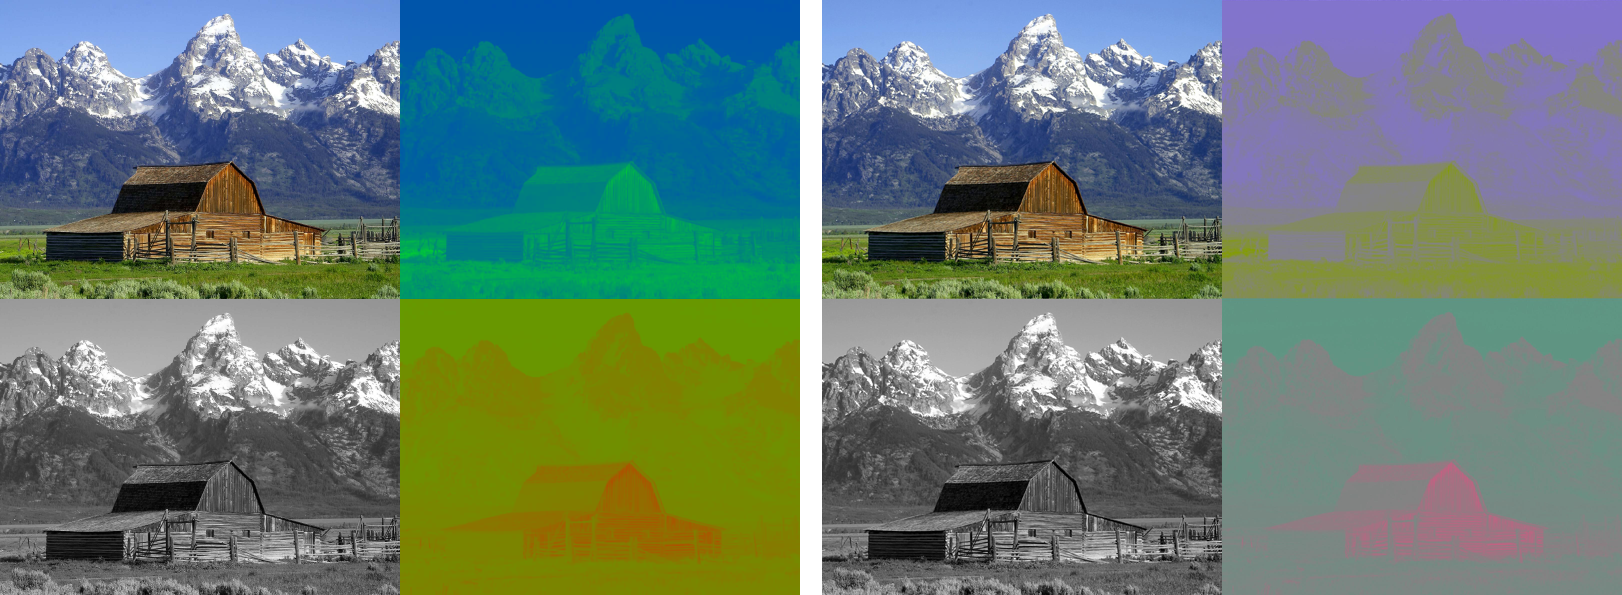
\includegraphics[width=\linewidth]{bilder/video_YUV-YCbCr}
\caption{Links die Aufteilung eines Bildes in die drei Kanäle Y, U und V. Auf der rechten Seite wurde das Bild in die drei Kanäle Y, Cb und Cr aufgeteilt. (Wikimedia Commons)}
\end{figure}

Da das menschliche Auge Farben im Vergleich zu Helligkeiten schlechter auflösen kann, wird eine Reduzierung in der Auflösung von Farbanteilen schlechter wahrgenommen. Wenn also der Y-Kanal vollständig übertragen wird, während die beiden Farbkanäle jeweils reduziert übertragen werden, ist optisch für den Menschen kein Unterschied in der Schärfe feststellbar. Diesen Umstand macht sich die Farbunterabtastung (engl. \emph{chroma subsampling}) zunutze, die im Folgenden und in Abbildung \ref{abb:video_farbunterabtastung} auf Seite \pageref{abb:video_farbunterabtastung} kurz erläutert wird.

Farbunterabtastung wird meist durch drei Zahlen dargestellt, die jeweils mit einem Doppelpunkt voneinander getrennt werden, wie beispielsweise 4:2:0. Die erste Ziffer bezieht sich auf die Luminanz, die als Referenz für die weiteren Ziffern verwendet wird. Es handelt sich dabei üblicherweise um eine Vier. 

Die zweite Ziffer beschreibt die horizontale Abtastung beider Farbkanäle im Verhältnis zur Luminanz. Handelt es sich dabei um eine Vier, wird die Chrominanz vollständig abgetastet, während eine Zwei bedeutet, dass die Chrominanz in der Horizontalen nur halb so oft, wie die Luminanz abgetastet wird. 

Die dritte Ziffer bezieht sich auf die vertikale Abtastung. Wenn die dritte Ziffer gleich der zweiten Ziffer ist, wird keine vertikale Farbunterabtastung angewendet. Wenn die dritte Ziffer eine Null ist, findet eine vertikale Farbunterabtastung im Verhältnis 2:1 beider Farbkanäle statt. 

Eine vierte Ziffer, die immer den gleichen Wert der ersten Ziffer hat, wird verwendet, wenn zusätzlich Transparenz kodiert werden soll.

%Eigene Umgebung für Grafik, um Tabellenzeilen extra zu formatieren
%Die Grafik besteht aus 3 x 4 Tabellen, mit gefärbten Zellen, um Pixel darzustellen
{
\renewcommand{\arraystretch}{1.0}% Schmalere Tabellenzeilen
\begin{figure}[!p]
\begin{center}
\begin{subfigure}{.3\textwidth}
%Kanal Y	
		\begin{tabular}{ccccccccc}
		\multirow{8}{*}{Y} & {\cellcolor[HTML]{AAAAAA}} & {\cellcolor[HTML]{AAAAAA}} & {\cellcolor[HTML]{ABABAB}} & {\cellcolor[HTML]{ABABAB}} & {\cellcolor[HTML]{BDBDBD}} & {\cellcolor[HTML]{9E9E9E}} & {\cellcolor[HTML]{A9A9A9}} & {\cellcolor[HTML]{ADADAD}} \\
		& {\cellcolor[HTML]{ACACAC}} & {\cellcolor[HTML]{ACACAC}} & {\cellcolor[HTML]{BBBBBB}} & {\cellcolor[HTML]{CDCDCD}} & {\cellcolor[HTML]{E3E3E3}} & {\cellcolor[HTML]{E9E9E9}} & {\cellcolor[HTML]{DEDEDE}} & {\cellcolor[HTML]{B1B1B1}} \\ 
		& {\cellcolor[HTML]{BABABA}} & {\cellcolor[HTML]{E4E4E4}} & {\cellcolor[HTML]{FAFAFA}} & {\cellcolor[HTML]{FCFCFC}} & {\cellcolor[HTML]{EDEDED}} & {\cellcolor[HTML]{D3D3D3}} & {\cellcolor[HTML]{DDDDDD}} & {\cellcolor[HTML]{D4D4D4}} \\ 
		& {\cellcolor[HTML]{B5B5B5}} & {\cellcolor[HTML]{DCDCDC}} & {\cellcolor[HTML]{DADADA}} & {\cellcolor[HTML]{D0D0D0}} & {\cellcolor[HTML]{A4A4A4}} & {\cellcolor[HTML]{A4A4A4}} & {\cellcolor[HTML]{BBBBBB}} & {\cellcolor[HTML]{ABABAB}} \\ 
		& {\cellcolor[HTML]{DBDBDB}} & {\cellcolor[HTML]{B0B0B0}} & {\cellcolor[HTML]{D6D6D6}} & {\cellcolor[HTML]{E3E3E3}} & {\cellcolor[HTML]{D7D7D7}} & {\cellcolor[HTML]{B6B6B6}} & {\cellcolor[HTML]{B4B4B4}} & {\cellcolor[HTML]{A7A7A7}} \\ 
		& {\cellcolor[HTML]{E3E3E3}} & {\cellcolor[HTML]{F6F6F6}} & {\cellcolor[HTML]{F0F0F0}} & {\cellcolor[HTML]{B9B9B9}} & {\cellcolor[HTML]{8E8E8E}} & {\cellcolor[HTML]{939393}} & {\cellcolor[HTML]{B6B6B6}} & {\cellcolor[HTML]{A6A6A6}} \\ 
		& {\cellcolor[HTML]{BDBDBD}} & {\cellcolor[HTML]{C8C8C8}} & {\cellcolor[HTML]{F7F7F7}} & {\cellcolor[HTML]{FCFCFC}} & {\cellcolor[HTML]{EFEFEF}} & {\cellcolor[HTML]{A0A0A0}} & {\cellcolor[HTML]{AAAAAA}}& {\cellcolor[HTML]{A5A5A5}} \\ 
		& {\cellcolor[HTML]{9E9E9E}} & {\cellcolor[HTML]{A2A2A2}} & {\cellcolor[HTML]{C9C9C9}} & {\cellcolor[HTML]{E2E2E2}} & {\cellcolor[HTML]{FBFBFB}} & {\cellcolor[HTML]{E0E0E0}} & {\cellcolor[HTML]{B1B1B1}} & {\cellcolor[HTML]{A8A8A8}} \\ 
	\end{tabular}\vspace{0.3cm}
	
%Kanal U
	\begin{tabular}{ccccccccc}
		\multirow{8}{*}{U} & {\cellcolor[HTML]{005AA5}} & {\cellcolor[HTML]{005AA5}} & {\cellcolor[HTML]{005EA1}} & {\cellcolor[HTML]{005EA1}} & {\cellcolor[HTML]{006897}} & {\cellcolor[HTML]{00758A}} & {\cellcolor[HTML]{006F90}} & {\cellcolor[HTML]{00619E}} \\
		& {\cellcolor[HTML]{0059A6}} & {\cellcolor[HTML]{005EA1}} & {\cellcolor[HTML]{006A95}} & {\cellcolor[HTML]{00748B}} & {\cellcolor[HTML]{007A85}} & {\cellcolor[HTML]{007D82}} & {\cellcolor[HTML]{007D82}} & {\cellcolor[HTML]{006996}} \\ 
		& {\cellcolor[HTML]{006996}} & {\cellcolor[HTML]{007788}} & {\cellcolor[HTML]{007D82}} & {\cellcolor[HTML]{007F80}} & {\cellcolor[HTML]{00807F}} & {\cellcolor[HTML]{007D82}} & {\cellcolor[HTML]{00807F}} & {\cellcolor[HTML]{007887}} \\ 
		& {\cellcolor[HTML]{007D82}} & {\cellcolor[HTML]{007E81}} & {\cellcolor[HTML]{007D82}} & {\cellcolor[HTML]{007E81}} & {\cellcolor[HTML]{007A85}} & {\cellcolor[HTML]{00748B}} & {\cellcolor[HTML]{007887}} & {\cellcolor[HTML]{007788}} \\ 
		& {\cellcolor[HTML]{00807F}} & {\cellcolor[HTML]{007A85}} & {\cellcolor[HTML]{007D82}} & {\cellcolor[HTML]{007E81}} & {\cellcolor[HTML]{007C83}} & {\cellcolor[HTML]{007689}} & {\cellcolor[HTML]{007689}} & {\cellcolor[HTML]{007788}} \\ 
		& {\cellcolor[HTML]{007B84}} & {\cellcolor[HTML]{007F80}} & {\cellcolor[HTML]{007D82}} & {\cellcolor[HTML]{007E81}} & {\cellcolor[HTML]{007689}} & {\cellcolor[HTML]{00748B}} & {\cellcolor[HTML]{007986}} & {\cellcolor[HTML]{007A85}} \\ 
		& {\cellcolor[HTML]{007689}} & {\cellcolor[HTML]{007C83}} & {\cellcolor[HTML]{007F80}} & {\cellcolor[HTML]{00827D}} & {\cellcolor[HTML]{007F80}} & {\cellcolor[HTML]{007A85}} & {\cellcolor[HTML]{007C83}}& {\cellcolor[HTML]{007986}} \\ 
		& {\cellcolor[HTML]{00748B}} & {\cellcolor[HTML]{007A85}} & {\cellcolor[HTML]{007C83}} & {\cellcolor[HTML]{007C83}} & {\cellcolor[HTML]{00807F}} & {\cellcolor[HTML]{007F80}} & {\cellcolor[HTML]{00807F}} & {\cellcolor[HTML]{007A85}} \\ 
	\end{tabular}\vspace{0.3cm}

%Kanal V
	\begin{tabular}{ccccccccc}
		\multirow{8}{*}{V} & {\cellcolor[HTML]{699600}} & {\cellcolor[HTML]{699600}} & {\cellcolor[HTML]{689700}} & {\cellcolor[HTML]{6D9200}} & {\cellcolor[HTML]{758A00}} & {\cellcolor[HTML]{7A8500}} & {\cellcolor[HTML]{788700}} & {\cellcolor[HTML]{6C9300}} \\
		& {\cellcolor[HTML]{689700}} & {\cellcolor[HTML]{6D9200}} & {\cellcolor[HTML]{748B00}} & {\cellcolor[HTML]{788700}} & {\cellcolor[HTML]{7D8200}} & {\cellcolor[HTML]{807F00}} & {\cellcolor[HTML]{7F8000}} & {\cellcolor[HTML]{748B00}} \\ 
		& {\cellcolor[HTML]{738C00}} & {\cellcolor[HTML]{7A8500}} & {\cellcolor[HTML]{7D8200}} & {\cellcolor[HTML]{7D8200}} & {\cellcolor[HTML]{7C8300}} & {\cellcolor[HTML]{7C8300}} & {\cellcolor[HTML]{7F8000}} & {\cellcolor[HTML]{778800}} \\ 
		& {\cellcolor[HTML]{7E8100}} & {\cellcolor[HTML]{817E00}} & {\cellcolor[HTML]{817E00}} & {\cellcolor[HTML]{7F8000}} & {\cellcolor[HTML]{7C8300}} & {\cellcolor[HTML]{7A8500}} & {\cellcolor[HTML]{7F8000}} & {\cellcolor[HTML]{7A8500}} \\ 
		& {\cellcolor[HTML]{7F8000}} & {\cellcolor[HTML]{7F8000}} & {\cellcolor[HTML]{807F00}} & {\cellcolor[HTML]{7F8000}} & {\cellcolor[HTML]{7F8000}} & {\cellcolor[HTML]{7E8100}} & {\cellcolor[HTML]{7F8000}} & {\cellcolor[HTML]{7D8200}} \\ 
		& {\cellcolor[HTML]{7C8300}} & {\cellcolor[HTML]{7E8100}} & {\cellcolor[HTML]{7F8000}} & {\cellcolor[HTML]{7C8300}} & {\cellcolor[HTML]{798600}} & {\cellcolor[HTML]{7A8500}} & {\cellcolor[HTML]{7D8200}} & {\cellcolor[HTML]{7F8000}} \\ 
		& {\cellcolor[HTML]{7B8400}} & {\cellcolor[HTML]{7E8100}} & {\cellcolor[HTML]{7F8000}} & {\cellcolor[HTML]{807F00}} & {\cellcolor[HTML]{7F8000}} & {\cellcolor[HTML]{7C8300}} & {\cellcolor[HTML]{7D8200}}& {\cellcolor[HTML]{7F8000}} \\ 
		& {\cellcolor[HTML]{7B8400}} & {\cellcolor[HTML]{7D8200}} & {\cellcolor[HTML]{7D8200}} & {\cellcolor[HTML]{807F00}} & {\cellcolor[HTML]{807F00}} & {\cellcolor[HTML]{7F8000}} & {\cellcolor[HTML]{7E8100}} & {\cellcolor[HTML]{7F8000}} \\ 
	\end{tabular}\vspace{0.3cm}

%Alles
	\begin{tabular}{ccccccccc}
		\multirow{8}{*}{A} & {\cellcolor[HTML]{8AAEEC}} & {\cellcolor[HTML]{8AAEEB}} & {\cellcolor[HTML]{89B1E6}} & {\cellcolor[HTML]{90ADE6}} & {\cellcolor[HTML]{AEBDE5}} & {\cellcolor[HTML]{969FB0}} & {\cellcolor[HTML]{9EAAC5}} & {\cellcolor[HTML]{92B1E3}} \\
		& {\cellcolor[HTML]{8AB0EF}} & {\cellcolor[HTML]{91AFE6}} & {\cellcolor[HTML]{AABDE0}} & {\cellcolor[HTML]{C1CFE1}} & {\cellcolor[HTML]{DFE4EC}} & {\cellcolor[HTML]{E9E9ED}} & {\cellcolor[HTML]{DCDEE2}} & {\cellcolor[HTML]{A0B2D7}} \\ 
		& {\cellcolor[HTML]{A8BBE1}} & {\cellcolor[HTML]{DCE5F2}} & {\cellcolor[HTML]{F6FCFE}} & {\cellcolor[HTML]{F8FEFB}} & {\cellcolor[HTML]{E8F0EC}} & {\cellcolor[HTML]{CDD5D7}} & {\cellcolor[HTML]{DBDEDB}} & {\cellcolor[HTML]{C8D8E0}} \\ 
		& {\cellcolor[HTML]{B2B6B9}} & {\cellcolor[HTML]{DDDBDE}} & {\cellcolor[HTML]{DCD9DE}} & {\cellcolor[HTML]{CED0D2}} & {\cellcolor[HTML]{9EA5AC}} & {\cellcolor[HTML]{9CA4B7}} & {\cellcolor[HTML]{B9B9C7}} & {\cellcolor[HTML]{A3ACB9}} \\ 
		& {\cellcolor[HTML]{D9DCD9}} & {\cellcolor[HTML]{AEAFB9}} & {\cellcolor[HTML]{D6D5DA}} & {\cellcolor[HTML]{E2E3E4}} & {\cellcolor[HTML]{D5D7DD}} & {\cellcolor[HTML]{B3B4C5}} & {\cellcolor[HTML]{B3B2C5}} & {\cellcolor[HTML]{A3A6B5}} \\ 
		& {\cellcolor[HTML]{DDE5EA}} & {\cellcolor[HTML]{F3F7F6}} & {\cellcolor[HTML]{EFF0F3}} & {\cellcolor[HTML]{B3BCBB}} & {\cellcolor[HTML]{84909E}} & {\cellcolor[HTML]{8B93A7}} & {\cellcolor[HTML]{B1B6C0}} & {\cellcolor[HTML]{A5A5AF}} \\ 
		& {\cellcolor[HTML]{B6BDCD}} & {\cellcolor[HTML]{C5C9CD}} & {\cellcolor[HTML]{F6F8F8}} & {\cellcolor[HTML]{FBFDF6}} & {\cellcolor[HTML]{EDF0EF}} & {\cellcolor[HTML]{9BA1A8}} & {\cellcolor[HTML]{A6ABB0}}& {\cellcolor[HTML]{A4A4AF}} \\ 
		& {\cellcolor[HTML]{989EB2}} & {\cellcolor[HTML]{9EA2AA}} & {\cellcolor[HTML]{C5CACF}} & {\cellcolor[HTML]{E1E1E6}} & {\cellcolor[HTML]{FBFBF9}} & {\cellcolor[HTML]{DFE1E1}} & {\cellcolor[HTML]{AEB3B0}} & {\cellcolor[HTML]{A6A7B1}} \\ 
	\end{tabular}
  \caption{4:4:4}
\end{subfigure}\hspace{0.65cm}
\begin{subfigure}{.3\textwidth}
%Kanal Y	
		\begin{tabular}{cccccccc}
		{\cellcolor[HTML]{AAAAAA}} & {\cellcolor[HTML]{AAAAAA}} & {\cellcolor[HTML]{ABABAB}} & {\cellcolor[HTML]{ABABAB}} & {\cellcolor[HTML]{BDBDBD}} & {\cellcolor[HTML]{9E9E9E}} & {\cellcolor[HTML]{A9A9A9}} & {\cellcolor[HTML]{ADADAD}} \\
		{\cellcolor[HTML]{ACACAC}} & {\cellcolor[HTML]{ACACAC}} & {\cellcolor[HTML]{BBBBBB}} & {\cellcolor[HTML]{CDCDCD}} & {\cellcolor[HTML]{E3E3E3}} & {\cellcolor[HTML]{E9E9E9}} & {\cellcolor[HTML]{DEDEDE}} & {\cellcolor[HTML]{B1B1B1}} \\ 
		{\cellcolor[HTML]{BABABA}} & {\cellcolor[HTML]{E4E4E4}} & {\cellcolor[HTML]{FAFAFA}} & {\cellcolor[HTML]{FCFCFC}} & {\cellcolor[HTML]{EDEDED}} & {\cellcolor[HTML]{D3D3D3}} & {\cellcolor[HTML]{DDDDDD}} & {\cellcolor[HTML]{D4D4D4}} \\ 
		{\cellcolor[HTML]{B5B5B5}} & {\cellcolor[HTML]{DCDCDC}} & {\cellcolor[HTML]{DADADA}} & {\cellcolor[HTML]{D0D0D0}} & {\cellcolor[HTML]{A4A4A4}} & {\cellcolor[HTML]{A4A4A4}} & {\cellcolor[HTML]{BBBBBB}} & {\cellcolor[HTML]{ABABAB}} \\ 
		{\cellcolor[HTML]{DBDBDB}} & {\cellcolor[HTML]{B0B0B0}} & {\cellcolor[HTML]{D6D6D6}} & {\cellcolor[HTML]{E3E3E3}} & {\cellcolor[HTML]{D7D7D7}} & {\cellcolor[HTML]{B6B6B6}} & {\cellcolor[HTML]{B4B4B4}} & {\cellcolor[HTML]{A7A7A7}} \\ 
		{\cellcolor[HTML]{E3E3E3}} & {\cellcolor[HTML]{F6F6F6}} & {\cellcolor[HTML]{F0F0F0}} & {\cellcolor[HTML]{B9B9B9}} & {\cellcolor[HTML]{8E8E8E}} & {\cellcolor[HTML]{939393}} & {\cellcolor[HTML]{B6B6B6}} & {\cellcolor[HTML]{A6A6A6}} \\ 
		{\cellcolor[HTML]{BDBDBD}} & {\cellcolor[HTML]{C8C8C8}} & {\cellcolor[HTML]{F7F7F7}} & {\cellcolor[HTML]{FCFCFC}} & {\cellcolor[HTML]{EFEFEF}} & {\cellcolor[HTML]{A0A0A0}} & {\cellcolor[HTML]{AAAAAA}}& {\cellcolor[HTML]{A5A5A5}} \\ 
		{\cellcolor[HTML]{9E9E9E}} & {\cellcolor[HTML]{A2A2A2}} & {\cellcolor[HTML]{C9C9C9}} & {\cellcolor[HTML]{E2E2E2}} & {\cellcolor[HTML]{FBFBFB}} & {\cellcolor[HTML]{E0E0E0}} & {\cellcolor[HTML]{B1B1B1}} & {\cellcolor[HTML]{A8A8A8}} \\ 
	\end{tabular}\vspace{0.3cm}
	
%Kanal U
	\begin{tabular}{cccccccc}
		{\cellcolor[HTML]{005AA5}} & {\cellcolor[HTML]{FFFFFF}} & {\cellcolor[HTML]{005EA1}} & {\cellcolor[HTML]{FFFFFF}} & {\cellcolor[HTML]{006897}} & {\cellcolor[HTML]{FFFFFF}} & {\cellcolor[HTML]{006F90}} & {\cellcolor[HTML]{FFFFFF}} \\
		{\cellcolor[HTML]{0059A6}} & {\cellcolor[HTML]{FFFFFF}} & {\cellcolor[HTML]{006A95}} & {\cellcolor[HTML]{FFFFFF}} & {\cellcolor[HTML]{007A85}} & {\cellcolor[HTML]{FFFFFF}} & {\cellcolor[HTML]{007D82}} & {\cellcolor[HTML]{FFFFFF}} \\ 
		{\cellcolor[HTML]{006996}} & {\cellcolor[HTML]{FFFFFF}} & {\cellcolor[HTML]{007D82}} & {\cellcolor[HTML]{FFFFFF}} & {\cellcolor[HTML]{00807F}} & {\cellcolor[HTML]{FFFFFF}} & {\cellcolor[HTML]{00807F}} & {\cellcolor[HTML]{FFFFFF}} \\ 
		{\cellcolor[HTML]{007D82}} & {\cellcolor[HTML]{FFFFFF}} & {\cellcolor[HTML]{007D82}} & {\cellcolor[HTML]{FFFFFF}} & {\cellcolor[HTML]{007A85}} & {\cellcolor[HTML]{FFFFFF}} & {\cellcolor[HTML]{007887}} & {\cellcolor[HTML]{FFFFFF}} \\ 
		{\cellcolor[HTML]{00807F}} & {\cellcolor[HTML]{FFFFFF}} & {\cellcolor[HTML]{007D82}} & {\cellcolor[HTML]{FFFFFF}} & {\cellcolor[HTML]{007C83}} & {\cellcolor[HTML]{FFFFFF}} & {\cellcolor[HTML]{007689}} & {\cellcolor[HTML]{FFFFFF}} \\ 
		{\cellcolor[HTML]{007B84}} & {\cellcolor[HTML]{FFFFFF}} & {\cellcolor[HTML]{007D82}} & {\cellcolor[HTML]{FFFFFF}} & {\cellcolor[HTML]{007689}} & {\cellcolor[HTML]{FFFFFF}} & {\cellcolor[HTML]{007986}} & {\cellcolor[HTML]{FFFFFF}} \\ 
		{\cellcolor[HTML]{007689}} & {\cellcolor[HTML]{FFFFFF}} & {\cellcolor[HTML]{007F80}} & {\cellcolor[HTML]{FFFFFF}} & {\cellcolor[HTML]{007F80}} & {\cellcolor[HTML]{FFFFFF}} & {\cellcolor[HTML]{007C83}} & {\cellcolor[HTML]{FFFFFF}} \\ 
		{\cellcolor[HTML]{00748B}} & {\cellcolor[HTML]{FFFFFF}} & {\cellcolor[HTML]{007C83}} & {\cellcolor[HTML]{FFFFFF}} & {\cellcolor[HTML]{00807F}} & {\cellcolor[HTML]{FFFFFF}} & {\cellcolor[HTML]{00807F}} & {\cellcolor[HTML]{FFFFFF}} \\ 
	\end{tabular}\vspace{0.3cm}

%Kanal V
	\begin{tabular}{cccccccc}
		{\cellcolor[HTML]{699600}} & {\cellcolor[HTML]{FFFFFF}} & {\cellcolor[HTML]{689700}} & {\cellcolor[HTML]{FFFFFF}} & {\cellcolor[HTML]{758A00}} & {\cellcolor[HTML]{FFFFFF}} & {\cellcolor[HTML]{788700}} & {\cellcolor[HTML]{FFFFFF}} \\
		{\cellcolor[HTML]{689700}} & {\cellcolor[HTML]{FFFFFF}} & {\cellcolor[HTML]{748B00}} & {\cellcolor[HTML]{FFFFFF}} & {\cellcolor[HTML]{7D8200}} & {\cellcolor[HTML]{FFFFFF}} & {\cellcolor[HTML]{7F8000}} & {\cellcolor[HTML]{FFFFFF}} \\ 
		{\cellcolor[HTML]{738C00}} & {\cellcolor[HTML]{FFFFFF}} & {\cellcolor[HTML]{7D8200}} & {\cellcolor[HTML]{FFFFFF}} & {\cellcolor[HTML]{7C8300}} & {\cellcolor[HTML]{FFFFFF}} & {\cellcolor[HTML]{7F8000}} & {\cellcolor[HTML]{FFFFFF}} \\ 
		{\cellcolor[HTML]{7E8100}} & {\cellcolor[HTML]{FFFFFF}} & {\cellcolor[HTML]{817E00}} & {\cellcolor[HTML]{FFFFFF}} & {\cellcolor[HTML]{7C8300}} & {\cellcolor[HTML]{FFFFFF}} & {\cellcolor[HTML]{7F8000}} & {\cellcolor[HTML]{FFFFFF}} \\ 
		{\cellcolor[HTML]{7F8000}} & {\cellcolor[HTML]{FFFFFF}} & {\cellcolor[HTML]{807F00}} & {\cellcolor[HTML]{FFFFFF}} & {\cellcolor[HTML]{7F8000}} & {\cellcolor[HTML]{FFFFFF}} & {\cellcolor[HTML]{7F8000}} & {\cellcolor[HTML]{FFFFFF}} \\ 
		{\cellcolor[HTML]{7C8300}} & {\cellcolor[HTML]{FFFFFF}} & {\cellcolor[HTML]{7F8000}} & {\cellcolor[HTML]{FFFFFF}} & {\cellcolor[HTML]{798600}} & {\cellcolor[HTML]{FFFFFF}} & {\cellcolor[HTML]{7D8200}} & {\cellcolor[HTML]{FFFFFF}} \\ 
		{\cellcolor[HTML]{7B8400}} & {\cellcolor[HTML]{FFFFFF}} & {\cellcolor[HTML]{7F8000}} & {\cellcolor[HTML]{FFFFFF}} & {\cellcolor[HTML]{7F8000}} & {\cellcolor[HTML]{FFFFFF}} & {\cellcolor[HTML]{7D8200}} & {\cellcolor[HTML]{FFFFFF}} \\ 
		{\cellcolor[HTML]{7B8400}} & {\cellcolor[HTML]{FFFFFF}} & {\cellcolor[HTML]{7D8200}} & {\cellcolor[HTML]{FFFFFF}} & {\cellcolor[HTML]{807F00}} & {\cellcolor[HTML]{FFFFFF}} & {\cellcolor[HTML]{7E8100}} & {\cellcolor[HTML]{FFFFFF}} \\ 
	\end{tabular}\vspace{0.3cm}

%Alles
	\begin{tabular}{cccccccc}
	{\cellcolor[HTML]{90ABE9}} & {\cellcolor[HTML]{90ABE9}} & {\cellcolor[HTML]{90AEE3}} & {\cellcolor[HTML]{90AEE3}} & {\cellcolor[HTML]{B2BCE4}} & {\cellcolor[HTML]{8F9EC6}} & {\cellcolor[HTML]{A0A9C4}} & {\cellcolor[HTML]{A4ADC7}} \\
	{\cellcolor[HTML]{91ADEC}} & {\cellcolor[HTML]{91ADEC}} & {\cellcolor[HTML]{ADBBDE}} & {\cellcolor[HTML]{C0CDEC}} & {\cellcolor[HTML]{DFE3EB}} & {\cellcolor[HTML]{E6EAF0}} & {\cellcolor[HTML]{DCDEE2}} & {\cellcolor[HTML]{AFB1B5}} \\
	{\cellcolor[HTML]{ACBAE0}} & {\cellcolor[HTML]{D8E5FF}} & {\cellcolor[HTML]{F7FBFD}} & {\cellcolor[HTML]{F9FDFF}} & {\cellcolor[HTML]{E9EFEC}} & {\cellcolor[HTML]{CED6D2}} & {\cellcolor[HTML]{DBDEDB}} & {\cellcolor[HTML]{D2D5D2}} \\
	{\cellcolor[HTML]{B3B6B9}} & {\cellcolor[HTML]{DADDDF}} & {\cellcolor[HTML]{DCD9DE}} & {\cellcolor[HTML]{D2CFD4}} & {\cellcolor[HTML]{A0A5AC}} & {\cellcolor[HTML]{A0A5AC}} & {\cellcolor[HTML]{B9B9C7}} & {\cellcolor[HTML]{A9A9B7}} \\
	{\cellcolor[HTML]{DADCDA}} & {\cellcolor[HTML]{AEB1AE}} & {\cellcolor[HTML]{D6D5DA}} & {\cellcolor[HTML]{E3E2E6}} & {\cellcolor[HTML]{D5D7DD}} & {\cellcolor[HTML]{B4B6BC}} & {\cellcolor[HTML]{B3B2C5}} & {\cellcolor[HTML]{A6A5B8}} \\
	{\cellcolor[HTML]{DEE4E9}} & {\cellcolor[HTML]{F1F7FA}} & {\cellcolor[HTML]{F0F0F3}} & {\cellcolor[HTML]{B8B9BC}} & {\cellcolor[HTML]{868F9D}} & {\cellcolor[HTML]{8C94A1}} & {\cellcolor[HTML]{B3B6C0}} & {\cellcolor[HTML]{A1A6B0}} \\
	{\cellcolor[HTML]{B8BDCD}} & {\cellcolor[HTML]{C3C8D5}} & {\cellcolor[HTML]{F6F7F7}} & {\cellcolor[HTML]{FBFCFC}} & {\cellcolor[HTML]{EDF0EF}} & {\cellcolor[HTML]{9EA1A0}} & {\cellcolor[HTML]{A7ABB0}} & {\cellcolor[HTML]{A1A6AB}} \\
	{\cellcolor[HTML]{999DB1}} & {\cellcolor[HTML]{999DB1}} & {\cellcolor[HTML]{C6CACF}} & {\cellcolor[HTML]{DFE2E6}} & {\cellcolor[HTML]{FBFBFA}} & {\cellcolor[HTML]{E0E0DE}} & {\cellcolor[HTML]{AFB3B0}} & {\cellcolor[HTML]{	A5AAA7}} \\
	\end{tabular}
  \caption{4:2:2}
\end{subfigure}
\begin{subfigure}{.3\textwidth}
%Kanal Y	
		\begin{tabular}{cccccccc}
		{\cellcolor[HTML]{AAAAAA}} & {\cellcolor[HTML]{AAAAAA}} & {\cellcolor[HTML]{ABABAB}} & {\cellcolor[HTML]{ABABAB}} & {\cellcolor[HTML]{BDBDBD}} & {\cellcolor[HTML]{9E9E9E}} & {\cellcolor[HTML]{A9A9A9}} & {\cellcolor[HTML]{ADADAD}} \\
		{\cellcolor[HTML]{ACACAC}} & {\cellcolor[HTML]{ACACAC}} & {\cellcolor[HTML]{BBBBBB}} & {\cellcolor[HTML]{CDCDCD}} & {\cellcolor[HTML]{E3E3E3}} & {\cellcolor[HTML]{E9E9E9}} & {\cellcolor[HTML]{DEDEDE}} & {\cellcolor[HTML]{B1B1B1}} \\ 
		{\cellcolor[HTML]{BABABA}} & {\cellcolor[HTML]{E4E4E4}} & {\cellcolor[HTML]{FAFAFA}} & {\cellcolor[HTML]{FCFCFC}} & {\cellcolor[HTML]{EDEDED}} & {\cellcolor[HTML]{D3D3D3}} & {\cellcolor[HTML]{DDDDDD}} & {\cellcolor[HTML]{D4D4D4}} \\ 
		{\cellcolor[HTML]{B5B5B5}} & {\cellcolor[HTML]{DCDCDC}} & {\cellcolor[HTML]{DADADA}} & {\cellcolor[HTML]{D0D0D0}} & {\cellcolor[HTML]{A4A4A4}} & {\cellcolor[HTML]{A4A4A4}} & {\cellcolor[HTML]{BBBBBB}} & {\cellcolor[HTML]{ABABAB}} \\ 
		{\cellcolor[HTML]{DBDBDB}} & {\cellcolor[HTML]{B0B0B0}} & {\cellcolor[HTML]{D6D6D6}} & {\cellcolor[HTML]{E3E3E3}} & {\cellcolor[HTML]{D7D7D7}} & {\cellcolor[HTML]{B6B6B6}} & {\cellcolor[HTML]{B4B4B4}} & {\cellcolor[HTML]{A7A7A7}} \\ 
		{\cellcolor[HTML]{E3E3E3}} & {\cellcolor[HTML]{F6F6F6}} & {\cellcolor[HTML]{F0F0F0}} & {\cellcolor[HTML]{B9B9B9}} & {\cellcolor[HTML]{8E8E8E}} & {\cellcolor[HTML]{939393}} & {\cellcolor[HTML]{B6B6B6}} & {\cellcolor[HTML]{A6A6A6}} \\ 
		{\cellcolor[HTML]{BDBDBD}} & {\cellcolor[HTML]{C8C8C8}} & {\cellcolor[HTML]{F7F7F7}} & {\cellcolor[HTML]{FCFCFC}} & {\cellcolor[HTML]{EFEFEF}} & {\cellcolor[HTML]{A0A0A0}} & {\cellcolor[HTML]{AAAAAA}}& {\cellcolor[HTML]{A5A5A5}} \\ 
		{\cellcolor[HTML]{9E9E9E}} & {\cellcolor[HTML]{A2A2A2}} & {\cellcolor[HTML]{C9C9C9}} & {\cellcolor[HTML]{E2E2E2}} & {\cellcolor[HTML]{FBFBFB}} & {\cellcolor[HTML]{E0E0E0}} & {\cellcolor[HTML]{B1B1B1}} & {\cellcolor[HTML]{A8A8A8}} \\ 
	\end{tabular}\vspace{0.3cm}
	
%Kanal U
	\begin{tabular}{cccccccc}
		{\cellcolor[HTML]{005AA5}} & {\cellcolor[HTML]{FFFFFF}} & {\cellcolor[HTML]{005EA1}} & {\cellcolor[HTML]{FFFFFF}} & {\cellcolor[HTML]{006897}} & {\cellcolor[HTML]{FFFFFF}} & {\cellcolor[HTML]{006F90}} & {\cellcolor[HTML]{FFFFFF}} \\
		{\cellcolor[HTML]{FFFFFF}} & {\cellcolor[HTML]{FFFFFF}} & {\cellcolor[HTML]{FFFFFF}} & {\cellcolor[HTML]{FFFFFF}} & {\cellcolor[HTML]{FFFFFF}} & {\cellcolor[HTML]{FFFFFF}} & {\cellcolor[HTML]{FFFFFF}} & {\cellcolor[HTML]{FFFFFF}} \\ 
		{\cellcolor[HTML]{006996}} & {\cellcolor[HTML]{FFFFFF}} & {\cellcolor[HTML]{007D82}} & {\cellcolor[HTML]{FFFFFF}} & {\cellcolor[HTML]{00807F}} & {\cellcolor[HTML]{FFFFFF}} & {\cellcolor[HTML]{00807F}} & {\cellcolor[HTML]{FFFFFF}} \\ 
		{\cellcolor[HTML]{FFFFFF}} & {\cellcolor[HTML]{FFFFFF}} & {\cellcolor[HTML]{FFFFFF}} & {\cellcolor[HTML]{FFFFFF}} & {\cellcolor[HTML]{FFFFFF}} & {\cellcolor[HTML]{FFFFFF}} & {\cellcolor[HTML]{FFFFFF}} & {\cellcolor[HTML]{FFFFFF}} \\ 
		{\cellcolor[HTML]{00807F}} & {\cellcolor[HTML]{FFFFFF}} & {\cellcolor[HTML]{007D82}} & {\cellcolor[HTML]{FFFFFF}} & {\cellcolor[HTML]{007C83}} & {\cellcolor[HTML]{FFFFFF}} & {\cellcolor[HTML]{007689}} & {\cellcolor[HTML]{FFFFFF}} \\ 
		{\cellcolor[HTML]{FFFFFF}} & {\cellcolor[HTML]{FFFFFF}} & {\cellcolor[HTML]{FFFFFF}} & {\cellcolor[HTML]{FFFFFF}} & {\cellcolor[HTML]{FFFFFF}} & {\cellcolor[HTML]{FFFFFF}} & {\cellcolor[HTML]{FFFFFF}} & {\cellcolor[HTML]{FFFFFF}} \\ 
		{\cellcolor[HTML]{007689}} & {\cellcolor[HTML]{FFFFFF}} & {\cellcolor[HTML]{007F80}} & {\cellcolor[HTML]{FFFFFF}} & {\cellcolor[HTML]{007F80}} & {\cellcolor[HTML]{FFFFFF}} & {\cellcolor[HTML]{007C83}} & {\cellcolor[HTML]{FFFFFF}} \\ 
		{\cellcolor[HTML]{FFFFFF}} & {\cellcolor[HTML]{FFFFFF}} & {\cellcolor[HTML]{FFFFFF}} & {\cellcolor[HTML]{FFFFFF}} & {\cellcolor[HTML]{FFFFFF}} & {\cellcolor[HTML]{FFFFFF}} & {\cellcolor[HTML]{FFFFFF}} & {\cellcolor[HTML]{FFFFFF}} \\ 
	\end{tabular}\vspace{0.3cm}

%Kanal V
	\begin{tabular}{cccccccc}
		{\cellcolor[HTML]{699600}} & {\cellcolor[HTML]{FFFFFF}} & {\cellcolor[HTML]{689700}} & {\cellcolor[HTML]{FFFFFF}} & {\cellcolor[HTML]{758A00}} & {\cellcolor[HTML]{FFFFFF}} & {\cellcolor[HTML]{788700}} & {\cellcolor[HTML]{FFFFFF}} \\
		{\cellcolor[HTML]{FFFFFF}} & {\cellcolor[HTML]{FFFFFF}} & {\cellcolor[HTML]{FFFFFF}} & {\cellcolor[HTML]{FFFFFF}} & {\cellcolor[HTML]{FFFFFF}} & {\cellcolor[HTML]{FFFFFF}} & {\cellcolor[HTML]{FFFFFF}} & {\cellcolor[HTML]{FFFFFF}} \\ 
		{\cellcolor[HTML]{738C00}} & {\cellcolor[HTML]{FFFFFF}} & {\cellcolor[HTML]{7D8200}} & {\cellcolor[HTML]{FFFFFF}} & {\cellcolor[HTML]{7C8300}} & {\cellcolor[HTML]{FFFFFF}} & {\cellcolor[HTML]{7F8000}} & {\cellcolor[HTML]{FFFFFF}} \\ 
		{\cellcolor[HTML]{FFFFFF}} & {\cellcolor[HTML]{FFFFFF}} & {\cellcolor[HTML]{FFFFFF}} & {\cellcolor[HTML]{FFFFFF}} & {\cellcolor[HTML]{FFFFFF}} & {\cellcolor[HTML]{FFFFFF}} & {\cellcolor[HTML]{FFFFFF}} & {\cellcolor[HTML]{FFFFFF}} \\ 
		{\cellcolor[HTML]{7F8000}} & {\cellcolor[HTML]{FFFFFF}} & {\cellcolor[HTML]{807F00}} & {\cellcolor[HTML]{FFFFFF}} & {\cellcolor[HTML]{7F8000}} & {\cellcolor[HTML]{FFFFFF}} & {\cellcolor[HTML]{7F8000}} & {\cellcolor[HTML]{FFFFFF}} \\ 
		{\cellcolor[HTML]{FFFFFF}} & {\cellcolor[HTML]{FFFFFF}} & {\cellcolor[HTML]{FFFFFF}} & {\cellcolor[HTML]{FFFFFF}} & {\cellcolor[HTML]{FFFFFF}} & {\cellcolor[HTML]{FFFFFF}} & {\cellcolor[HTML]{FFFFFF}} & {\cellcolor[HTML]{FFFFFF}} \\ 
		{\cellcolor[HTML]{7B8400}} & {\cellcolor[HTML]{FFFFFF}} & {\cellcolor[HTML]{7F8000}} & {\cellcolor[HTML]{FFFFFF}} & {\cellcolor[HTML]{7F8000}} & {\cellcolor[HTML]{FFFFFF}} & {\cellcolor[HTML]{7D8200}} & {\cellcolor[HTML]{FFFFFF}} \\ 
		{\cellcolor[HTML]{FFFFFF}} & {\cellcolor[HTML]{FFFFFF}} & {\cellcolor[HTML]{FFFFFF}} & {\cellcolor[HTML]{FFFFFF}} & {\cellcolor[HTML]{FFFFFF}} & {\cellcolor[HTML]{FFFFFF}} & {\cellcolor[HTML]{FFFFFF}} & {\cellcolor[HTML]{FFFFFF}} \\ 
	\end{tabular}\vspace{0.3cm}

%Alles
	\begin{tabular}{cccccccc}
	{\cellcolor[HTML]{90ABE9}} & {\cellcolor[HTML]{90ABE9}} & {\cellcolor[HTML]{90AEE3}} & {\cellcolor[HTML]{90AEE3}} & {\cellcolor[HTML]{B2BCE4}} & {\cellcolor[HTML]{8F9EC6}} & {\cellcolor[HTML]{A0A9C4}} & {\cellcolor[HTML]{A4ADC7}} \\
	{\cellcolor[HTML]{93ADEB}} & {\cellcolor[HTML]{93ADEB}} & {\cellcolor[HTML]{A1BEF0}} & {\cellcolor[HTML]{B4D1FE}} & {\cellcolor[HTML]{DAE3FF}} & {\cellcolor[HTML]{E2E9FF}} & {\cellcolor[HTML]{D6DFF2}} & {\cellcolor[HTML]{A8B1CA}} \\
	{\cellcolor[HTML]{ACBAE0}} & {\cellcolor[HTML]{D8E5FF}} & {\cellcolor[HTML]{F7FBFD}} & {\cellcolor[HTML]{F9FDFF}} & {\cellcolor[HTML]{E9EFEC}} & {\cellcolor[HTML]{CED6D2}} & {\cellcolor[HTML]{DBDEDB}} & {\cellcolor[HTML]{D2D5D2}} \\
	{\cellcolor[HTML]{A6B5DB}} & {\cellcolor[HTML]{CFDDF9}} & {\cellcolor[HTML]{D6DCDE}} & {\cellcolor[HTML]{CCD2D4}} & {\cellcolor[HTML]{9FA7A3}} & {\cellcolor[HTML]{9FA7A3}} & {\cellcolor[HTML]{B9BCB9}} & {\cellcolor[HTML]{A9ACA9}} \\
	{\cellcolor[HTML]{DADCDA}} & {\cellcolor[HTML]{AEB1AE}} & {\cellcolor[HTML]{D6D5DA}} & {\cellcolor[HTML]{E3E2E6}} & {\cellcolor[HTML]{D5D7DD}} & {\cellcolor[HTML]{B4B6BC}} & {\cellcolor[HTML]{B3B2C5}} & {\cellcolor[HTML]{A6A5B8}} \\
	{\cellcolor[HTML]{E2E4E2}} & {\cellcolor[HTML]{F5F7F5}} & {\cellcolor[HTML]{F0EFF3}} & {\cellcolor[HTML]{B9B8BD}} & {\cellcolor[HTML]{8C8E94}} & {\cellcolor[HTML]{919399}} & {\cellcolor[HTML]{B5B4C6}} & {\cellcolor[HTML]{A5A4B7}} \\
	{\cellcolor[HTML]{B8BDCD}} & {\cellcolor[HTML]{C3C8D5}} & {\cellcolor[HTML]{F6F7F7}} & {\cellcolor[HTML]{FBFCFC}} & {\cellcolor[HTML]{EDF0EF}} & {\cellcolor[HTML]{9EA1A0}} & {\cellcolor[HTML]{A7ABB0}} & {\cellcolor[HTML]{A1A6AB}} \\
	{\cellcolor[HTML]{979EAE}} & {\cellcolor[HTML]{9BA2B2}} & {\cellcolor[HTML]{C8CACA}} & {\cellcolor[HTML]{E1E3E3}} & {\cellcolor[HTML]{FAFCFC}} & {\cellcolor[HTML]{DEE1E0}} & {\cellcolor[HTML]{AEB1B5}} & {\cellcolor[HTML]{A5A9AE}} \\
	\end{tabular}
  \caption{4:2:0}
\end{subfigure}
\end{center}
  \caption{Schematische Darstellung der Farbunterabtastung. Bei 4:4:4 werden die Informationen aller drei Kanäle vollständig abgetastet. Bei 4:2:2 wird der Y-Kanal vollständig und im U- und V-Kanal jeweils nur jeder zweite Pixel jeder Zeile gelesen. Bei 4:2:0 wird der Y-Kanal ebenfalls vollständig gelesen, während die Farbkanäle U und V jeweils nur zur Hälfte in der Horizontalen und in der Vertikalen gelesen werden, also nur jeder zweite Pixel in jeder zweiten Zeile. Werden die drei Kanäle zusammengerechnet, weisen die Gesamtbilder optisch kaum sichtbare Unterschiede auf.}
\label{abb:video_farbunterabtastung}
\end{figure}
}%Ende Umgebung für die Grafik

\label{video-datenrate}
\subparagraph{Datenrate} Die Datenrate, gibt an wie viele Daten in einer bestimmten Zeitspanne übertragen oder gelesen werden. Bei digitalen Videos wird die Datenrate in Bits pro Sekunde gemessen, weshalb hier auch von Bitrate gesprochen wird. 

Wenn eine konstante Bitrate (\emph{constant bitrate}, CBR) angewendet wird, wird pro Sekunde immer die gleiche Datenmenge übertragen, was zur Folge haben kann, dass komplexe Bildinhalte an Qualität verlieren. Bei der Anwendung einer variablen Bitrate (\emph{variable bitrate}, VBR) variiert die Menge der übertragenen Daten je nach Komplexität des Bildinhaltes, was eine höhere Bildqualität zur Folge hat. Da bei der VBR ruhige und einfache Bildübergänge und -inhalte mit einer niedrigen Datenrate gespeichert werden, kann der Speicherplatzverbrauch verringert werden.

In den meisten Codecs wird eine variable Bitrate verwendet.
%XXXInterlaced vs. Progressiv?

\pagebreak
\paragraph{Praxis} In diesem Abschnitt sind Hinweise zum Umgang mit Videodateien gesammelt. Es gibt Erläuterungen mit Literatur- und Programmhinweisen über die Ansicht und Extraktion von Metadaten, die Wiedergabe und die Transcodierung von Videos. Zur Digitalisierung von Filmmaterial können nur allgemeine Hinweise gegeben werden.

\subparagraph{Metadaten} Die technischen Metadaten der Containerdatei sind in der Regel in dessen Header gespeichert. Weitere Metadaten können in den Video- und Audiostreams gespeichert sein. Diese Daten können von verschiedenen Programmen ausgelesen werden. Ein Programm, das mit vielen Formaten umgehen kann und auch den Export von Metadaten in eine gesonderte Datei erlaubt ist MediaInfo.

\begin{figure}[!htp]
  \begin{center}
    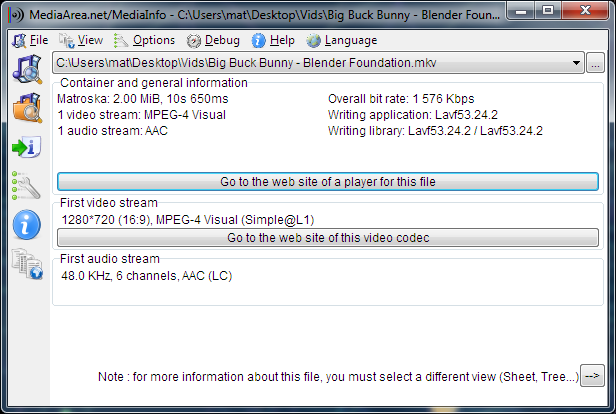
\includegraphics[width=0.9\textwidth]{bilder/video_mediainfo}
  \end{center}
  \caption{Die Übersichtsseite von MediaInfo für eine analysierte MKV-Datei.}
\end{figure}

Zu den Exportformaten gehören PBCore und EBUCore. Es handelt sich dabei um Metadatenschemata, die speziell für Film und Ton von Public Broadcasting in den USA, beziehungsweise von der European Broadcasting Union (EBU) entwickelt wurden. Die Moving Pictures Experts Group (MPEG) hat MPEG-7 für die Dokumentation von Multimediadateien entwickelt, der insbesondere zur Erweiterung der anderen MPEG-Standards gedacht ist.

\begin{flushleft}
	MediaInfo: \urllist{https://mediaarea.net/MediaInfo}
	PBCore: \urllist{http://pbcore.org/}
	EBUCore: \urllist{https://tech.ebu.ch/MetadataEbuCore}
	MPEG-7: \urllist{http://mpeg.chiariglione.org/standards/mpeg-7}
\end{flushleft}

\subparagraph{Wiedergabeprogramme} Jedes Betriebssystem hat meist schon ein Programm für die Wiedergabe von Videodateien vorinstalliert. Jedoch können diese Programme nur mit einer begrenzten Auswahl von Containerformaten und Codecs umgehen. Codecs können nachträglich installiert werden, wobei aber auf Kompatibilität mit dem Wiedergabeprogramm geachtet werden muss.

Ein Programm, das mit allen hier vorgestellten Formaten und Codecs umgehen kann, ist der VLC media player. Unter der einfach gehaltenen Oberfläche verbirgt sich eine Vielzahl an Funktionalitäten und das Programm gibt es für alle gängigen Betriebssysteme. 

\begin{figure}[!htp]
  \begin{center}
    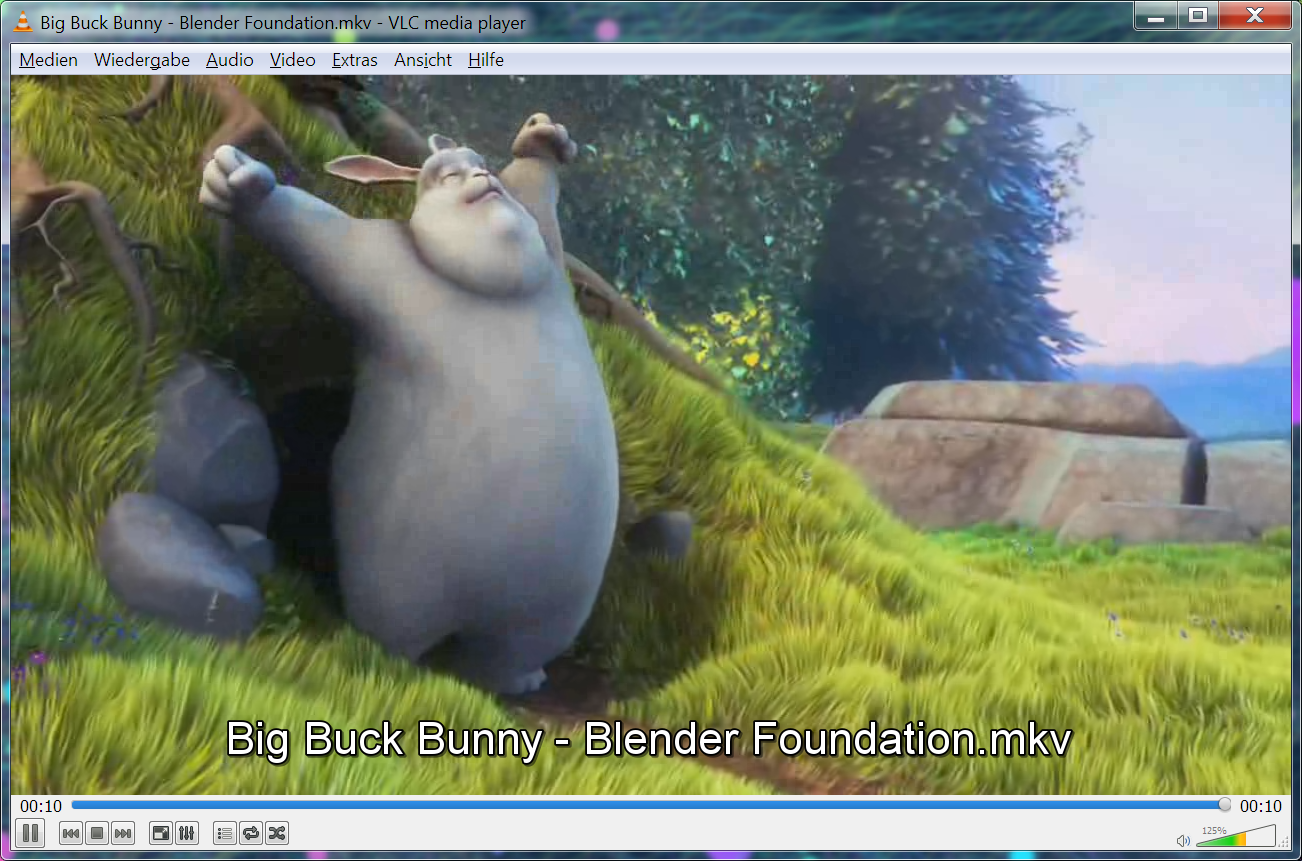
\includegraphics[width=0.9\textwidth]{bilder/video_vlc}
  \end{center}
	\caption{VLC media player}
\end{figure}

\begin{flushleft}
	VLC media player von VideoLAN: \urllist{http://www.videolan.org/vlc/index.html}
\end{flushleft}

\subparagraph{Transcodierung} Für die Transcodierung von einem Codec in einen weiteren gibt es einige frei verfügbare Programme, wie beispielsweise der bereits vorgestellt VLC media player, der eine leicht verständliche grafische Oberfläche anbietet. Auch das frei verfügbare Programm Handbrake ist für mehrere Betriebssysteme verfügbar und bietet eine grafische Oberfläche, ist jedoch im Gegensatz zu VLC nur auf die Transcodierung spezialisiert.

Für fortgeschrittene Anwender ist das ebenfalls frei verfügbare FFmpeg zu empfehlen, das komplexere und detailliertere Transcodierungsoptionen erlaubt und auch von der Kommandozeile aus gesteuert werden kann. 

\begin{flushleft}
	VLC media player von VideoLAN: \urllist{http://www.videolan.org/vlc/index.html}
	Handbrake: \urllist{https://handbrake.fr/}
	FFmpeg: \urllist{https://www.ffmpeg.org/}
\end{flushleft}


\subparagraph{Digitalisierung und Aufnahme} Die Digitalisierung von Film- und Videomaterial ist angesichts der beinahe unüberschaubaren Menge an analogen Film- und Videoformaten nicht Gegenstand dieser Empfehlungen. 

Im Allgemeinen sollte darauf geachtet werden, dass das originale analoge Material weiterhin erhalten bleibt. Bei der Digitalisierung muss auf größtmögliche Qualität und Originaltreue geachtet werden, wobei vor allem Farbwiedergabe und Seitenverhältnis unverändert bleiben sollten. Die Konsultierung eines darauf spezialisierten Archivs oder Dienstleisters ist hierbei ratsam.

Die Aufnahmen neuer Videos sollten digital erfolgen, da diese die Analogtechnik inzwischen an Qualität meist übertrifft. Dabei sollten die Audiodaten in linearem PCM oder FLAC aufgenommen werden und die Videodaten entweder unkomprimiert, als FLAC oder in möglichst hochqualitativem H.264/MPEG-4 AVC gespeichert werden. Von der DFG gibt es weitere Hinweise in der Handreichung \href{http://www.dfg.de/download/pdf/foerderung/grundlagen_dfg_foerderung/informationen_fachwissenschaften/geisteswissenschaften/standards_sprachkorpora.pdf}{\emph{Empfehlungen zu datentechnischen Standards und Tools bei der Erhebung von Sprachkorpora}}.


\paragraph{Quellen}
\begin{flushleft}
Archaeology Data Service, Digital Video: A Guide to Good Practice \urllist{http://guides.archaeologydataservice.ac.uk/g2gp/Video_Toc}

W. Bergmeyer, Multimedia/Komplexe Applikationen, in: H. Neuroth -- A. Oßwald -- R. Scheffel -- S. Strathmann -- K. Huth (Hrsg.) nestor Handbuch. Eine kleine Enzyklopädie der digitalen Langzeitarchiverung. Version 2.3 (2010) Kap. 17.4 \urllist{http://www.nestor.sub.uni-goettingen.de/handbuch}

G. Blood, Refining Conversion Contract Specifications: Determining Suitable Digital Video Formats for Medium-term Storage. (2011) \urllist{http://www.digitizationguidelines.gov/audio-visual/documents/IntrmMastVidFormatRecs_20111001.pdf}

P. Bubestinger -- H. Lewetz -- M. Jaks, The archivist's video codec and container FAQ (2013) \urllist{http://download.das-werkstatt.com/pb/mthk/info/video/FAQ-digital_video_archiving.html}

P. Bubestinger -- H. Lewetz -- M. Jaks, Comparing video codecs and containers for archives (2015) \urllist{http://download.das-werkstatt.com/pb/mthk/info/video/comparison_video_codecs_containers.html}

B. Devlin, MXF -- The Material Exchange Format, in: EBU Technical Review (2002) \urllist{http://www.ebu.ch/en/technical/trev/trev_291-devlin.pdf}

B. Devlin, MXF. What is it, how does it work, and why hasn't it solved the world's problems yet? (2012) \urllist{http://www.tvtechnology.com/research-&-standards/0114/mxf/262167}

DFG Handreichung Empfehlungen zu datentechnischen Standards und Tools bei der Erhebung von Sprachkorpora\urllist{http://www.dfg.de/download/pdf/foerderung/grundlagen_dfg_foerderung/informationen_fachwissenschaften/geisteswissenschaften/standards_sprachkorpora.pdf}

V. Ernst -- J. Kepier -- J. Renz -- A. Romeyke -- T. Bähr, Leitfaden für die digitale Langzeitarchivierung audiovisueller Medien (2016) \urllist{http://nbn-resolving.de/urn:nbn:de:0008-2016102107}

equasys (Hrsg.), Color Formats (2015) \urllist{http://www.equasys.de/colorformat.html}

Koordinationsstelle für die dauerhafte Archivierung elektronischer Unterlagen (Hrsg.) Katalog archivischer Dateiformate: Videodaten \urllist{http://kost-ceco.ch/wiki/whelp/KaD/pages/Video.html}

C. Lacinak, A Primer on Codecs for Moving Image and Sound Archives. 10 Recommendations for Codec Selection and Management (2010) \urllist{http://www.avpreserve.com/wp-content/uploads/2010/04/AVPS_Codec_Primer.pdf}

E. Lorrain, A short guide to choosing a digital format for video archiving masters (2014) \urllist{https://www.scart.be/?q=en/content/short-guide-choosing-digital-format-video-archiving-masters}

Memoriav (Hrsg.), Digitale Archivierung von Film und Video: Grundlagen und Orientierung (2015) \urllist{http://memoriav.ch/wp-content/uploads/2015/04/Empfehlungen_Digitale_-Archivierung_Version1.0.pdf}

G. Pearson -- M. Gill, An Evaluation of Motion JPEG 2000 for Video Archiving, in: Proceedings IS\&T Archiving 2005 vom 26. bis 29. April in Washington, D.C. (Washington, D.C. 2005) 237-243 \urllist{http://dancearchivalproject.wikispaces.asu.edu/file/view/MJ2_video_archiving.pdf}

C. Poynton, Chroma subsampling notation (2008) \urllist{http://www.poynton.com/PDFs/Chroma_subsampling_notation.pdf}

D. Sauter, Video, In: H. Neuroth -- A. Oßwald -- R. Scheffel -- S. Strathmann -- K. Huth (Hrsg.) nestor Handbuch. Eine kleine Enzyklopädie der digitalen Langzeitarchiverung. Version 2.3 (2010) Kap. 17.5 \urllist{http://www.nestor.sub.uni-goettingen.de/handbuch}

K. van Malssen, Digital Video Preservation and Oral History, in: D. Boyd -- S. Cohen -- B. Rakerd -- D. Rehberger (Hrsg.) Oral History in the Digital Age (Washington, D.C. 2012) \urllist{http://ohda.matrix.msu.edu/2012/06/digital-video-preservation-and-oral-history/}

FFV1 vs other formats for preservation, Diskussion in Google Gruppe \urllist{https://groups.google.com/forum/\#!topic/archivematica/HulV96gJ0go}

What is a FOURCC? (englisch, 04. 2016) \urllist{http://www.fourcc.org/fourcc.php}

Wikipedia Bitrate (deutsch, 04. 2016) \urllist{https://de.wikipedia.org/wiki/Bitrate}

Wikipedia MPEG-4 (englisch, 04. 2016) \urllist{https://en.wikipedia.org/wiki/MPEG-4}

Filmausschnitte aus Big Buck Bunny von der Blender Foundation (2008) \urllist{http://www.bigbuckbunny.org/}

\quelltyp{Formatspezifikationen}
Matroska: \urllist{https://www.matroska.org/}
Matroska: Library of Congress \urllist{http://www.digitalpreservation.gov/formats/fdd/fdd000342.shtml}
Matroska: IETF CELLAR Charter \urllist{https://datatracker.ietf.org/doc/charter-ietf-cellar/}
Motion JPEG 2000: \urllist{https://jpeg.org/jpeg2000/}
Motion JPEG 2000: Library of Congress \urllist{http://www.digitalpreservation.gov/formats/fdd/fdd000127.shtml}
Motion JPEG 2000: RFC 3745 \urllist{http://www.ietf.org/rfc/rfc3745.txt}
Motion JPEG 2000: R. Kromer, Glossareintrag JPEG 2000 \urllist{http://avpres.net/Glossar/JPEG2000.html}
MPEG: \urllist{http://mpeg.chiariglione.org/}
MPEG-1: \urllist{http://mpeg.chiariglione.org/standards/mpeg-1}
MPEG-1: Library of Congress \urllist{http://www.digitalpreservation.gov/formats/fdd/fdd000035.shtml}
MPEG-2: \urllist{http://mpeg.chiariglione.org/standards/mpeg-2}
MPEG-2: Library of Congress \urllist{http://www.digitalpreservation.gov/formats/fdd/fdd000335.shtml}
MPEG-4: \urllist{http://mpeg.chiariglione.org/standards/mpeg-4}
MPEG-4: Library of Congress \urllist{http://www.digitalpreservation.gov/formats/fdd/fdd000037.shtml}
MPEG-4: RFC 4337 \urllist{http://www.ietf.org/rfc/rfc4337.txt}
MXF: SMPTE 377-1 \urllist{http://dx.doi.org/10.5594/SMPTE.ST377-1.2011}
MXF: Library of Congress \urllist{http://www.digitalpreservation.gov/formats/fdd/fdd000013.shtml}
MXF: RFC 4539 \urllist{http://www.ietf.org/rfc/rfc4539.txt}
FFV1: \urllist{http://www.ffmpeg.org/~michael/ffv1.html}

\quelltyp{Tools und Programme}
MediaInfo: \urllist{https://mediaarea.net/MediaInfo}
PBCore: \urllist{http://pbcore.org/}
EBUCore: \urllist{https://tech.ebu.ch/MetadataEbuCore}
MPEG-7: \urllist{http://mpeg.chiariglione.org/standards/mpeg-7}
VLC media player von VideoLAN: \urllist{http://www.videolan.org/vlc/index.html}
Handbrake: \urllist{https://handbrake.fr/}
FFmpeg: \urllist{https://www.ffmpeg.org/}
\end{flushleft}